% ============================================================
%  GSoC 2026 -- MetaCall -- MCP Support for Deploy & FaaS
%  Author : Swastik Prakash
%  Compile: xelatex -> xelatex (two passes for TOC)
% ============================================================
\documentclass[12pt, a4paper]{article}

% ---------- FONTS ----------
\usepackage{fontspec}
\setmainfont{Times New Roman}
\setsansfont{Arial}
\setmonofont{Courier New}

% ---------- LAYOUT ----------
\usepackage[
  top=2.5cm, bottom=2.5cm,
  left=2.8cm, right=2.8cm,
  headheight=26pt
]{geometry}
\usepackage{setspace}
\setstretch{1.15}
\usepackage{parskip}
\setlength{\parindent}{0pt}

% ---------- COLOUR ----------
\usepackage[dvipsnames, table]{xcolor}
\definecolor{mcblue}{HTML}{1565C0}
\definecolor{mclight}{HTML}{E3F2FD}
\definecolor{mcgray}{HTML}{F5F5F5}
\definecolor{mcdark}{HTML}{1A1A2E}
\definecolor{mcaccent}{HTML}{0D47A1}
\definecolor{mcgold}{HTML}{F9A825}
\definecolor{mcgreen}{HTML}{2E7D32}
\definecolor{mcorange}{HTML}{E65100}
\definecolor{mcpurple}{HTML}{6A1B9A}
\definecolor{codebg}{HTML}{FAFAFA}
\definecolor{titlebg}{HTML}{0D1B2A}
\definecolor{linkblue}{HTML}{64B5F6}

% ---------- GRAPHICS ----------
\usepackage{graphicx}
\usepackage{float}
\usepackage{tikz}
\usetikzlibrary{
  shapes.geometric, arrows.meta, positioning,
  shadows, fit, backgrounds, calc,
  decorations.pathmorphing, patterns
}

% ---------- TABLES ----------
\usepackage{booktabs}
\usepackage{tabularx}
\usepackage{multirow}
\usepackage{colortbl}
\usepackage{array}

% ---------- CODE ----------
\usepackage{listings}
\lstdefinestyle{tsStyle}{
  backgroundcolor=\color{codebg},
  basicstyle=\ttfamily\footnotesize,
  keywordstyle=\color{mcblue}\bfseries,
  commentstyle=\color{gray}\itshape,
  stringstyle=\color{teal},
  numberstyle=\tiny\color{gray},
  numbers=left, stepnumber=1,
  frame=l, framerule=2pt, rulecolor=\color{mcblue},
  breaklines=true, captionpos=b, tabsize=2,
  showstringspaces=false,
  morekeywords={async,await,const,let,import,from,export,
    interface,type,string,number,boolean,void,Promise,Tool,Server}
}
\lstdefinestyle{pyStyle}{
  backgroundcolor=\color{codebg},
  basicstyle=\ttfamily\footnotesize,
  keywordstyle=\color{mcblue}\bfseries,
  commentstyle=\color{gray}\itshape,
  stringstyle=\color{teal},
  numbers=left, numberstyle=\tiny\color{gray}, stepnumber=1,
  frame=l, framerule=2pt, rulecolor=\color{mcgreen},
  breaklines=true, captionpos=b, tabsize=4,
  showstringspaces=false, language=Python
}
\lstset{style=tsStyle}

% ---------- HYPERLINKS ----------
\usepackage[
  colorlinks=true,
  linkcolor=mcblue,
  urlcolor=mcblue,
  citecolor=mcblue
]{hyperref}
\usepackage{xurl}
\urlstyle{same}

% ---------- SECTION STYLING ----------
\usepackage{titlesec}
\titleformat{\section}
  {\Large\bfseries\color{mcdark}}
  {\colorbox{mcblue}{\textcolor{white}{\;\thesection\;}}}{0.8em}{}
  [\vspace{2pt}\color{mcblue}\titlerule]
\titleformat{\subsection}
  {\large\bfseries\color{mcaccent}}
  {\thesubsection}{0.8em}{}
\titleformat{\subsubsection}
  {\normalsize\bfseries\color{mcdark}}
  {\thesubsubsection}{0.8em}{}

% ---------- HEADER / FOOTER ----------
\usepackage{fancyhdr}
\pagestyle{fancy}
\fancyhf{}
\fancyhead[L]{\small\textcolor{mcblue}{\textbf{GSoC 2026}}
  \textcolor{gray}{ | MetaCall MCP Support}}
\fancyhead[R]{\small\textcolor{gray}{Swastik Prakash}}
\fancyfoot[C]{%
  
\begin{tikzpicture}
    \node[fill=mcblue, text=white, rounded corners=3pt,
          inner xsep=6pt, inner ysep=2pt,
          font=\small\bfseries] {\thepage};
  \end{tikzpicture}%
}
\renewcommand{\headrulewidth}{0.6pt}
\renewcommand{\headrule}{\hbox to\headwidth{%
  \color{mcblue}\leaders\hrule height \headrulewidth\hfill}}

% ---------- CALLOUT BOXES ----------
\usepackage{tcolorbox}
\tcbuselibrary{skins, breakable}
\newtcolorbox{infobox}[1][]{
  enhanced, breakable,
  colback=mclight, colframe=mcblue,
  fonttitle=\bfseries\color{white}, coltitle=white,
  attach boxed title to top left={yshift=-2mm, xshift=4mm},
  boxed title style={colback=mcblue, rounded corners},
  title=#1, left=8pt, right=8pt, top=8pt, bottom=6pt, arc=3pt
}
\newtcolorbox{highlightbox}{
  enhanced,
  colback=mcblue!6, colframe=mcblue!70,
  left=8pt, right=8pt, top=6pt, bottom=6pt, arc=4pt,
  borderline west={3pt}{0pt}{mcblue}
}
\newtcolorbox{achievementbox}{
  enhanced,
  colback=mcgold!8, colframe=mcgold!70,
  left=8pt, right=8pt, top=6pt, bottom=6pt, arc=4pt,
  borderline west={3pt}{0pt}{mcgold}
}

% ---------- MISC ----------
\usepackage{enumitem}
\usepackage{amsmath}
\usepackage{microtype}
\usepackage{pifont}
\newcommand{\cmark}{\ding{51}}

% ============================================================
\begin{document}
% ============================================================

% ====== TITLE PAGE ======
\begin{titlepage}
  \pagecolor{titlebg}
  \color{white}
  \centering

  \vspace*{0.8cm}

  
\begin{tikzpicture}
    \draw[mcblue!50, line width=0.8pt] (-7,0) -- (7,0);
  \end{tikzpicture}

  \vspace{0.5cm}

  % GSoC badge
  
\begin{tikzpicture}
    \fill[mcblue!15, rounded corners=12pt]
      (-4.2,-0.7) rectangle (4.2, 0.7);
    \node[fill=mcblue, rounded corners=10pt,
          inner xsep=18pt, inner ysep=10pt,
          drop shadow={shadow xshift=1pt, shadow yshift=-2pt,
                       fill=black!40}] {
      \Large\bfseries\color{white} Google Summer of Code 2026
    };
    \foreach \x in {-3.6,-3.3,...,3.6} {
      \fill[mcgold!60] (\x, -1.0) circle (1pt);
    }
  \end{tikzpicture}

  \vspace{0.8cm}

  {\fontsize{26}{32}\selectfont\bfseries
    Implement Model Context Protocol\par}
  \vspace{4pt}
  {\fontsize{26}{32}\selectfont\bfseries
    (MCP) Support for\par}
  \vspace{4pt}
  {\fontsize{26}{32}\selectfont\bfseries
    MetaCall Deploy \& FaaS\par}

  \vspace{0.5cm}

  
\begin{tikzpicture}
    \draw[mcblue, line width=1.2pt] (-4,0) -- (-0.5,0);
    \fill[mcgold] (0,0) circle (3pt);
    \draw[mcblue, line width=1.2pt] (0.5,0) -- (4,0);
  \end{tikzpicture}

  \vspace{0.6cm}

  {\LARGE\bfseries Swastik Prakash\par}
  \vspace{4pt}
  {\normalsize B.Tech Computer Science Engineering\par}
  \vspace{2pt}
  {\normalsize Jaypee Institute of Information Technology, Noida\par}

  \vspace{0.5cm}

  {\small
    \href{mailto:swastikprakashofficial@gmail.com}{%
      \textcolor{linkblue}{\underline{swastikprakashofficial@gmail.com}}}%
  }\\[5pt]
  {\small
    \href{https://github.com/Swastik-Prakash1}{%
      \textcolor{linkblue}{\underline{github.com/Swastik-Prakash1}}}%
    \quad\textcolor{mcblue!50}{$|$}\quad
    \href{https://linkedin.com/in/swastik-prakash}{%
      \textcolor{linkblue}{\underline{linkedin.com/in/swastik-prakash}}}%
  }\\[5pt]
  {\small\textcolor{gray!70}{%
    +91 8081605787 \quad$\cdot$\quad Uttar Pradesh, India}}

  \vspace{0.7cm}

  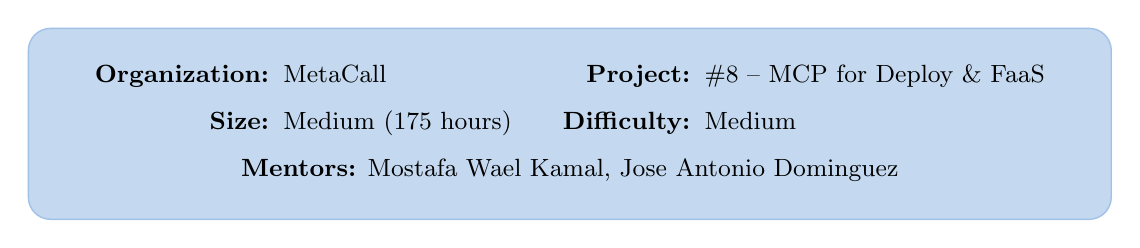
\begin{tikzpicture}
    \node[fill=mcblue!25, rounded corners=8pt,
      inner xsep=18pt, inner ysep=12pt,
      draw=mcblue!40, line width=0.5pt] {
  \color{black}\small
  \begin{tabular}{r@{\;\;}l@{\qquad}r@{\;\;}l}
        \textbf{Organization:} & MetaCall &
        \textbf{Project:} & \#8 -- MCP for Deploy \& FaaS \\[6pt]
        \textbf{Size:} & Medium (175 hours) &
        \textbf{Difficulty:} & Medium \\[6pt]
        \multicolumn{4}{c}{\textbf{Mentors:}
          Mostafa Wael Kamal, Jose Antonio Dominguez} \\
      \end{tabular}
    };
  \end{tikzpicture}

  \vspace{0.5cm}

  
\begin{tikzpicture}
    \draw[mcblue!50, line width=0.8pt] (-7,0) -- (7,0);
  \end{tikzpicture}

\end{titlepage}

\pagecolor{white}
\newpage

% ====== TOC ======
{
\pagestyle{fancy}
\tableofcontents
}
\vspace{1.5em}

% ============================================================
%  1. SYNOPSIS
% ============================================================
\newpage
\section{Synopsis}

\begin{highlightbox}
MetaCall is the only open-source polyglot runtime that lets developers
call functions across Python, JavaScript, TypeScript, Go, Rust, and more,
all seamlessly. This project makes MetaCall's FaaS platform
\textbf{AI-native} by building a production-grade \textbf{Model Context
Protocol (MCP) server}. Once complete, Claude, GitHub Copilot, and any
MCP-compatible AI assistant will be able to deploy, list, inspect, and
call serverless functions through plain English, right from VS Code or
any AI interface.
\end{highlightbox}

\vspace{0.6em}

This is not a theoretical proposal. I have \textbf{already built and
demonstrated} a working proof-of-concept MCP server that connects VS Code
GitHub Copilot to a local \texttt{metacall/faas} instance. I demoed it
live to MetaCall mentor \textbf{viferga}, who responded:
\emph{``awesome mate.''} Mentor \textbf{Mostafa Wael Kamal} has also
reviewed my work. This GSoC project takes that working foundation and
turns it into a production-grade, tested, documented, and officially
integrated tool for the entire MetaCall ecosystem.

MetaCall Core has 1,770+ GitHub stars, is written in C, supports
18 language ecosystems, and is licensed under Apache 2.0. MetaCall FaaS
is the TypeScript reimplementation powering
\texttt{dashboard.metacall.io} for local and cloud serverless
deployments. MetaCall Protocol provides shared TypeScript types across
the ecosystem. My MCP server sits on top of all three, giving AI
assistants a standardized way to interact with this entire stack.

% ============================================================
%  2. ABOUT ME
% ============================================================
\newpage
\section{About Me}

\subsection{Personal Information}

\begin{table}[H]
\centering
\begin{tabularx}{\textwidth}{>{\bfseries\color{mcdark}}l X}
  Full Name  & Swastik Prakash \\
  Email      & \href{mailto:swastikprakashofficial@gmail.com}%
               {swastikprakashofficial@gmail.com} \\
  GitHub     & \href{https://github.com/Swastik-Prakash1}%
               {github.com/Swastik-Prakash1} \\
  LinkedIn   & \href{https://linkedin.com/in/swastik-prakash}%
               {linkedin.com/in/swastik-prakash} \\
  Phone      & +91 8081605787 \\
  Location   & Uttar Pradesh, India \\
  University & Jaypee Institute of Information Technology, Noida \\
  Degree     & B.Tech, Computer Science Engineering (Expected 2027) \\
  Year       & 3rd year \\
  Timezone   & IST (UTC+5:30) \\
\end{tabularx}
\end{table}

\subsection{Education}

I am a 3rd-year B.Tech CSE student at JIIT Noida. My coursework includes
Machine Learning, Artificial Intelligence, Big Data Analytics, Data
Structures, and Algorithms. I consistently apply classroom learning to
real systems, whether it is building AI triage assistants, deploying NLP
pipelines, or solving algorithmic challenges under competitive
constraints.

\subsection{Competitive Programming and DSA}

\begin{achievementbox}
I have been deeply invested in Data Structures and Algorithms since my
second semester of first year. It started as curiosity and quickly became
the core of how I think about software. Today I am \textbf{ranked 3rd in
my entire college in DSA} and hold the \textbf{2nd position in AI/ML}
across all departments.
\end{achievementbox}

I maintain a dedicated GitHub repository where I archive well-thought-out
competitive programming solutions covering topics from graph algorithms
and dynamic programming to advanced data structures like segment trees,
tries, and balanced BSTs. Each solution is annotated with the approach,
complexity analysis, and edge cases I considered.

I have been practicing competitive programming consistently for over two
years now, and I plan to keep going. I regularly solve problems on
Codeforces, LeetCode, and CodeChef, and I actively prepare for technical
interviews because I genuinely enjoy the process of breaking down hard
problems into clean, efficient code. I have won multiple DSA competitions
at the college level and participate actively in inter-college coding
contests.

This background directly benefits my work on the MCP server. When I
built the proof-of-concept, the zip-and-upload pipeline for
\texttt{deploy\_local} required careful stream handling, buffering, and
async coordination. My instinct to think about edge cases and resource
management comes straight from years of competitive problem solving.

\subsection{Hackathon Achievement}

\begin{achievementbox}
\textbf{1st Place -- Build with Gemini $\times$ MLH, Zetech HackDay}
(International, 2026). Won a 12-hour AI hackathon powered by Google
Gemini and Major League Hacking with \textbf{MediMind}, my AI Clinical
Triage Assistant. Built a full multimodal system with persistent session
memory, vision model inference, context-aware multi-turn reasoning, and
emergency SOS Guardian Mode.
\href{https://devpost.com}{%
  \textcolor{mcblue}{[Devpost]}}
\end{achievementbox}

\subsection{Technical Skills}

\begin{table}[H]
\centering
\rowcolors{2}{mcgray}{white}
\begin{tabularx}{\textwidth}{>{\bfseries\color{mcdark}}l X}
  \toprule
  \rowcolor{mcblue!15}
  \textbf{Domain} & \textbf{Skills and Tools} \\
  \midrule
  Languages & Python, TypeScript/JavaScript, C++ \\
  DSA / CP  & Algorithm Design, Graph Theory, DP,
              Segment Trees, Tries, Competitive Programming \\
  AI / ML   & LLM Integration, RoBERTa, OpenAI API,
              Hugging Face, Transformers, Multimodal Pipelines \\
  Backend   & Flask, REST API design, Node.js v22, npm v10 \\
  DevOps    & Docker, GitHub Copilot (agent mode), VS Code,
              Git, GitHub Actions \\
  Cloud     & Google Cloud Platform, Oracle Cloud Infrastructure \\
  Protocols & MCP, HTTP, JSON, stdio/SSE transports \\
  \bottomrule
\end{tabularx}
\caption{Technical skills}
\end{table}

\subsection{Certifications}

\begin{itemize}[leftmargin=1.5em, itemsep=2pt]
  \item Oracle Certified AI Foundations Associate (OCI)
  \item Google Cloud Study Jam, Google Developer Student Clubs
  \item CDAC Noida, Bootcamp on Cloud Computing (FutureSkills PRIME)
\end{itemize}

\subsection{Selected Projects}

\subsubsection{MediMind -- AI Clinical Triage (1st Place, MLH Hackathon)}

Built a production-grade multimodal AI triage system with persistent
session memory, vision model inference, and context-aware multi-turn
clinical reasoning. Engineered a real-time SOS Guardian Mode with
emergency override, and implemented clinical SOAP report generation for
structured specialist handoff.
\textit{Stack: Python, Flask, Google Gemini, Multimodal Vision.}

\subsubsection{Should I? -- AI Trust Analysis System}

Built a scalable fake review detection system using fine-tuned RoBERTa
for real-time inference across 1,000+ reviews per product, with a
deterministic trust-scoring engine that aggregates linguistic and
behavioral anomalies.
\textit{Stack: Python, RoBERTa, NLP, Flask.}

\subsubsection{AI Interview Assistant}

Developed semantic similarity scoring using embeddings for rubric-aligned
response evaluation. Integrated speech signal processing and visual
features into a multimodal assessment framework.
\textit{Stack: Python, NLP, Speech Processing, ML.}

\subsubsection{Streaming-ML -- Algorithm Comparison for LLMs}

A research-oriented repository comparing different streaming algorithms
for large language models, combining competitive algorithm analysis with
practical ML engineering.
\textit{Stack: Python, ML Algorithms, Benchmarking.}

% ============================================================
%  3. PRE-GSoC CONTRIBUTIONS
% ============================================================
\newpage
\section{Pre-GSoC Contributions to MetaCall}

\begin{highlightbox}
I did not wait for GSoC to start contributing. Before writing this
proposal, I explored the codebase, submitted a pull request, found and
documented real bugs, and built a working MCP proof-of-concept that
earned praise from MetaCall's founder.
\end{highlightbox}

\subsection{PR \#200 -- metacall/deploy: Interactive Screen UX Fix}

\textbf{Issue:} \#154, ``feat: Any interactive screen should show:
Ctrl+C for cancel''

\textbf{Status:} Open PR (draft), reviewed positively, awaiting merge.

\begin{infobox}[Evidence Links -- PR \#200]
\begin{itemize}[leftmargin=1.2em, itemsep=4pt]
  \item \textbf{PR conversation (Discord):}
  \href{https://discord.com/channels/781987805974757426/1242205848453775412/1478742776773611712}
  {\nolinkurl{https://discord.com/channels/781987805974757426/1242205848453775412/1478742776773611712}}

  \item \textbf{PR result / maintainer feedback (Discord):}
  \href{https://discord.com/channels/781987805974757426/1242205848453775412/1478746380418678867}
  {\nolinkurl{https://discord.com/channels/781987805974757426/1242205848453775412/1478746380418678867}}

  \item \textbf{Pull Request (GitHub):}
  \href{https://github.com/metacall/deploy/pull/200}
  {\nolinkurl{https://github.com/metacall/deploy/pull/200}}
\end{itemize}
\end{infobox}

\subsection{MCP Server Proof-of-Concept}

\textbf{Repository:}
\href{https://github.com/Swastik-Prakash1/metacall-mcp}
{\nolinkurl{https://github.com/Swastik-Prakash1/metacall-mcp}}

\begin{infobox}[Evidence Links -- MCP Proof-of-Concept]
\begin{itemize}[leftmargin=1.2em, itemsep=4pt]
  \item \textbf{MCP working demo video (Discord):}
  \href{https://discord.com/channels/781987805974757426/1242205848453775412/1479423737110724651}
  {\nolinkurl{https://discord.com/channels/781987805974757426/1242205848453775412/1479423737110724651}}

  \item \textbf{MCP PR / discussion post (Discord):}
  \href{https://discord.com/channels/781987805974757426/1242205848453775412/1479329899180196011}
  {\nolinkurl{https://discord.com/channels/781987805974757426/1242205848453775412/1479329899180196011}}
\end{itemize}
\end{infobox}


Before submitting, I read the original closed PR \#173 and studied
maintainer \textbf{viferga's specific rejection feedback} line by line
to make sure my implementation addressed every concern.

\textbf{What I changed:}
\begin{itemize}[leftmargin=1.5em, itemsep=2pt]
  \item \textbf{Persistent screens} (\texttt{inspect.ts},
        \texttt{logs.ts}): Added a dimmed ``Press Ctrl+C to cancel.''
        hint inside the infinite/polling loops, exactly where viferga
        said it belongs.
  \item \textbf{List-type prompts} (\texttt{selection.ts}): Added an
        ``Exit'' option instead of Ctrl+C, following viferga's feedback
        that list prompts should offer a clean graceful exit.
\end{itemize}

The logic for both patterns as a flowchart:

\begin{figure}[H]
\centering
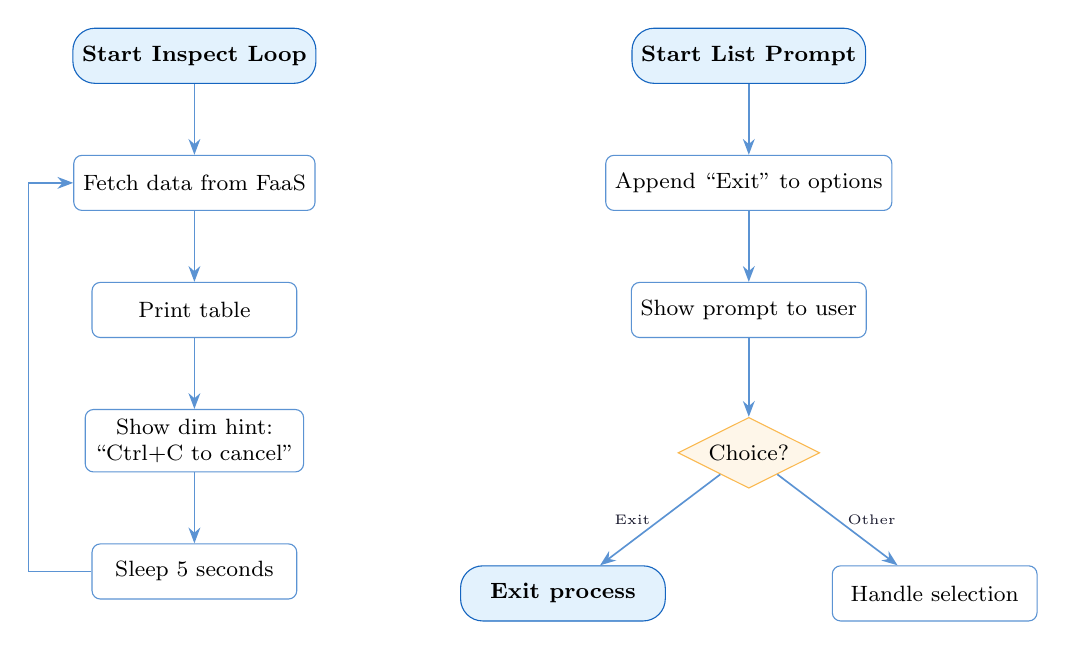
\begin{tikzpicture}[
  node distance=0.9cm,
  startstop/.style={rectangle, rounded corners=8pt,
    draw=mcblue, fill=mclight,
    minimum width=2.6cm, minimum height=0.7cm,
    align=center, font=\footnotesize\bfseries},
  process/.style={rectangle, rounded corners=3pt,
    draw=mcblue!70, fill=white,
    minimum width=2.6cm, minimum height=0.7cm,
    align=center, font=\footnotesize},
  decision/.style={diamond, draw=mcgold!80, fill=mcgold!10,
    minimum width=1.8cm, minimum height=0.9cm,
    align=center, font=\footnotesize,
    inner sep=1pt, aspect=2},
  arr/.style={-Stealth, semithick, color=mcblue!70},
  lbl/.style={font=\tiny, text=mcdark}
]
  % Left: Persistent Screen
  \node[startstop] (s1) {Start Inspect Loop};
  \node[process, below=of s1] (p1) {Fetch data from FaaS};
  \node[process, below=of p1] (p2) {Print table};
  \node[process, below=of p2] (p3) {Show dim hint:\\``Ctrl+C to cancel''};
  \node[process, below=of p3] (p4) {Sleep 5 seconds};
  \draw[arr] (s1) -- (p1);
  \draw[arr] (p1) -- (p2);
  \draw[arr] (p2) -- (p3);
  \draw[arr] (p3) -- (p4);
  \draw[arr] (p4.west) -- ++(-0.8,0) |- (p1.west);

  % Right: List Prompt
  \node[startstop, right=4cm of s1] (s2)
    {Start List Prompt};
  \node[process, below=of s2] (q1)
    {Append ``Exit'' to options};
  \node[process, below=of q1] (q2)
    {Show prompt to user};
  \node[decision, below=1cm of q2] (d1) {Choice?};
  \node[startstop, below left=1.2cm and 0.6cm of d1] (e1)
    {Exit process};
  \node[process, below right=1.2cm and 0.6cm of d1] (e2)
    {Handle selection};

  \draw[arr] (s2)  -- (q1);
  \draw[arr] (q1)  -- (q2);
  \draw[arr] (q2)  -- (d1);
  \draw[arr] (d1)  -- node[lbl, left]{Exit} (e1);
  \draw[arr] (d1)  -- node[lbl, right]{Other} (e2);
\end{tikzpicture}
\caption{Two UX patterns: persistent screen loop (left)
  and list prompt with Exit option (right)}
\end{figure}

The TypeScript implementation:

\begin{lstlisting}[caption={inspect.ts -- Ctrl+C hint},
  style=tsStyle]
p.printTable();
process.stdout.write(
  '\n\x1b[2m  Press Ctrl+C to cancel.\x1b[0m\n'
);
await sleep(5000);
\end{lstlisting}

\begin{lstlisting}[caption={selection.ts -- Exit option},
  style=tsStyle]
const EXIT_OPTION = 'Exit';
const handleExit = (value: string): void => {
  if (value === EXIT_OPTION) {
    process.stdout.write('\nExiting...\n');
    process.exit(0);
  }
};
\end{lstlisting}

\textbf{Testing:} Ran local FaaS with \texttt{docker compose up}, then
\texttt{node dist/index.js --dev --inspect}. Confirmed the dimmed hint
appeared. Sent a screenshot to viferga on Discord.

\newpage
\subsection{MCP Server Proof-of-Concept}

\textbf{Repository:}
\href{https://github.com/Swastik-Prakash1/metacall-mcp}%
{github.com/Swastik-Prakash1/metacall-mcp}

\textbf{Status:} Fully working. Demoed via video to viferga, who said
\textbf{``awesome mate.''} Shared with mentor Mostafa Wael Kamal.

I built a TypeScript MCP server that connects VS Code GitHub Copilot
to a local \texttt{metacall/faas} Docker instance. A developer types
plain English in Copilot Chat and can deploy, list, or call polyglot
serverless functions without touching a terminal.

\subsubsection{Architecture}

\begin{figure}[H]
\centering
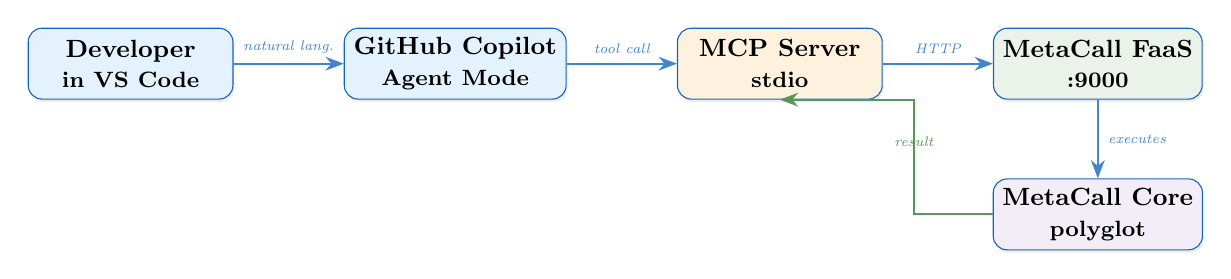
\begin{tikzpicture}[
  node distance=1cm and 1.4cm,
  box/.style={rectangle, draw=mcblue, fill=white,
              rounded corners=5pt,
              minimum width=2.6cm, minimum height=0.9cm,
              align=center, font=\small\bfseries,
              drop shadow={shadow xshift=0.5pt,
                           shadow yshift=-1pt, fill=gray!30}},
  arr/.style={-Stealth, thick, color=mcblue!80}
]
  \node[box, fill=mclight] (user)
    {Developer\\{\footnotesize in VS Code}};
  \node[box, fill=mclight, right=1.4cm of user] (copilot)
    {GitHub Copilot\\{\footnotesize Agent Mode}};
  \node[box, fill=mcgold!15, right=1.4cm of copilot] (mcp)
    {MCP Server\\{\footnotesize stdio}};
  \node[box, fill=mcgreen!10, right=1.4cm of mcp] (faas)
    {MetaCall FaaS\\{\footnotesize :9000}};
  \node[box, fill=mcpurple!8, below=1cm of faas] (core)
    {MetaCall Core\\{\footnotesize polyglot}};

  \draw[arr] (user) --
    node[above, font=\tiny\itshape]{natural lang.} (copilot);
  \draw[arr] (copilot) --
    node[above, font=\tiny\itshape]{tool call} (mcp);
  \draw[arr] (mcp) --
    node[above, font=\tiny\itshape]{HTTP} (faas);
  \draw[arr] (faas) --
    node[right, font=\tiny\itshape]{executes} (core);
  \draw[arr, mcgreen!80] (core.west) -- ++(-1,0) |-
    node[above, near start, font=\tiny\itshape]{result}
    (mcp.south);
\end{tikzpicture}
\caption{PoC architecture: Copilot to MetaCall FaaS via MCP}
\end{figure}

\subsubsection{Three Implemented MCP Tools}

\begin{table}[H]
\centering
\rowcolors{2}{mcgray}{white}
\begin{tabularx}{\textwidth}{>{\ttfamily\bfseries\footnotesize}p{3cm} X}
  \toprule
  \rowcolor{mcblue!15}
  \textbf{Tool} & \textbf{What it does} \\
  \midrule
  list\_deployments &
    Calls \texttt{GET /api/inspect}, returns all deployed
    functions with status, version, prefix \\
  deploy\_local &
    Zips directory, uploads via
    \texttt{POST /api/package/create},
    deploys via \texttt{POST /api/deploy/create} \\
  call\_function &
    Calls the function endpoint, returns the result \\
  \bottomrule
\end{tabularx}
\caption{MCP tools in the proof-of-concept}
\end{table}

The deploy workflow as a flowchart:

\begin{figure}[H]
\centering
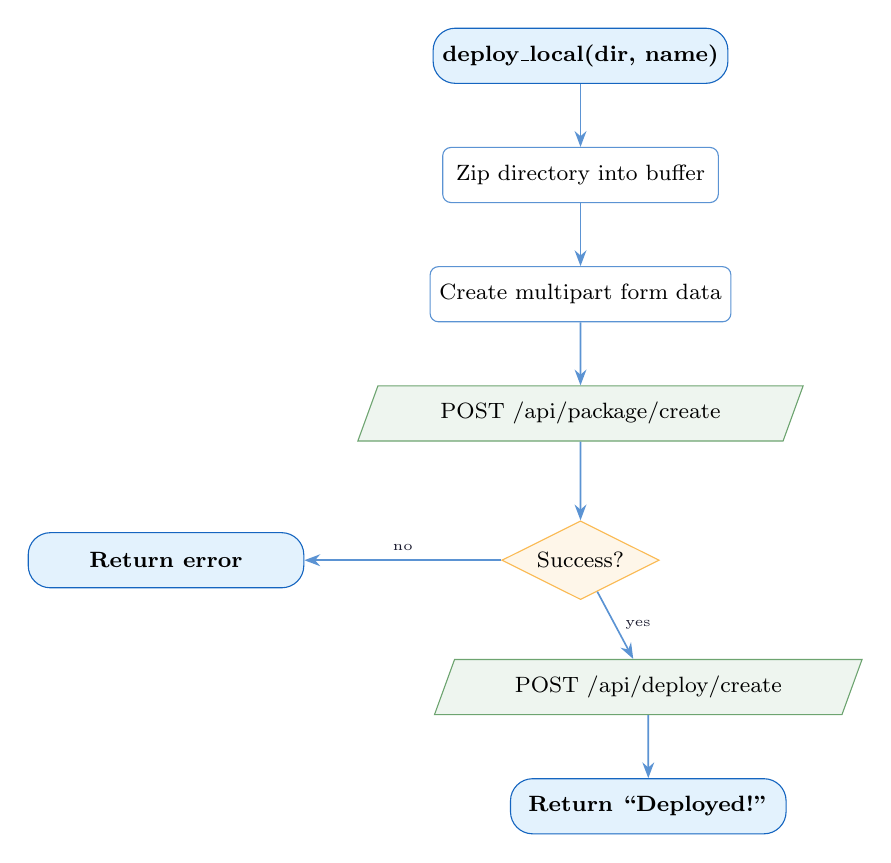
\begin{tikzpicture}[
  node distance=0.8cm,
  startstop/.style={rectangle, rounded corners=8pt,
    draw=mcblue, fill=mclight,
    minimum width=3.5cm, minimum height=0.7cm,
    align=center, font=\footnotesize\bfseries},
  process/.style={rectangle, rounded corners=3pt,
    draw=mcblue!70, fill=white,
    minimum width=3.5cm, minimum height=0.7cm,
    align=center, font=\footnotesize},
  decision/.style={diamond, draw=mcgold!80, fill=mcgold!10,
    minimum width=2cm, minimum height=1cm,
    align=center, font=\footnotesize,
    inner sep=1pt, aspect=2.2},
  io/.style={trapezium, trapezium left angle=70,
    trapezium right angle=110,
    draw=mcgreen!70, fill=mcgreen!8,
    minimum width=3cm, minimum height=0.7cm,
    align=center, font=\footnotesize},
  arr/.style={-Stealth, semithick, color=mcblue!70},
  lbl/.style={font=\tiny, text=mcdark}
]
  \node[startstop] (start)
    {deploy\_local(dir, name)};
  \node[process, below=of start] (zip)
    {Zip directory into buffer};
  \node[process, below=of zip] (form)
    {Create multipart form data};
  \node[io, below=of form] (upload)
    {POST /api/package/create};
  \node[decision, below=1cm of upload] (check)
    {Success?};
  \node[io, below right=1cm and 0cm of check] (deploy)
    {POST /api/deploy/create};
  \node[startstop, below=0.8cm of deploy] (done)
    {Return ``Deployed!''};
  \node[startstop, left=2.5cm of check] (fail)
    {Return error};

  \draw[arr] (start) -- (zip);
  \draw[arr] (zip)   -- (form);
  \draw[arr] (form)  -- (upload);
  \draw[arr] (upload) -- (check);
  \draw[arr] (check) -- node[lbl, right]{yes} (deploy);
  \draw[arr] (check) -- node[lbl, above]{no} (fail);
  \draw[arr] (deploy) -- (done);
\end{tikzpicture}
\caption{Flowchart: deploy\_local tool workflow}
\end{figure}

\subsubsection{Live Demo Transcript}

\begin{infobox}[Live Demo: Copilot Chat with metacall-mcp]
\texttt{User:} list my metacall deployments\\
\texttt{Copilot:} No deployments found.\\[4pt]
\texttt{User:} deploy the directory
  C:\textbackslash D\textbackslash Pro\textbackslash mc\textbackslash
  hello-test as hello-test\\
\texttt{Copilot:} Deployed successfully.\\[4pt]
\texttt{User:} list my metacall deployments\\
\texttt{Copilot:} hello-test (ready), version: v1,
  prefix: f889f5dee176\\[4pt]
\texttt{User:} call the hello function with name World\\
\texttt{Copilot:} ``Hello World from MetaCall!''
\end{infobox}

\begin{lstlisting}[caption={hello-test Python function deployed via MCP},
  style=pyStyle]
# main.py
def hello(name):
    return f'Hello {name} from MetaCall!'
\end{lstlisting}

\subsection{Bug Investigation in metacall/faas}

While setting up the local FaaS for testing, I discovered and documented
two bugs:

\begin{enumerate}[leftmargin=1.5em, itemsep=4pt]
  \item \textbf{CRLF line endings in \texttt{test/test.sh}} causing
        \texttt{exec: not found} errors inside Linux Docker containers.
        Fixed by converting to LF and adding
        \texttt{.gitattributes}: \texttt{*.sh text eol=lf}.

  \item \textbf{Race condition in
        \texttt{src/controller/package.ts}}:
        busboy's \texttt{finish} event fires before the async
        \texttt{fs.promises.mkdtemp} completes, causing
        \texttt{resource.blob} to be \texttt{undefined}.
        This blocks all package deployment tests.
        I documented the root cause and reported it.
\end{enumerate}

% ============================================================
%  4. PROJECT UNDERSTANDING
% ============================================================
\newpage
\section{Project Understanding}

\subsection{What Is MetaCall?}

MetaCall is an extensible, embeddable, cross-platform polyglot runtime.
It lets you call functions written in one programming language from
another: Python from JavaScript, Node.js from Python, Rust from
TypeScript, all transparently.

The core runtime (\texttt{metacall/core}) is written in C, has 1,770+
GitHub stars, 220 forks, and supports 18 language ecosystems. It is
licensed under Apache 2.0.

\subsection{MetaCall Ecosystem}

\begin{figure}[H]
\centering
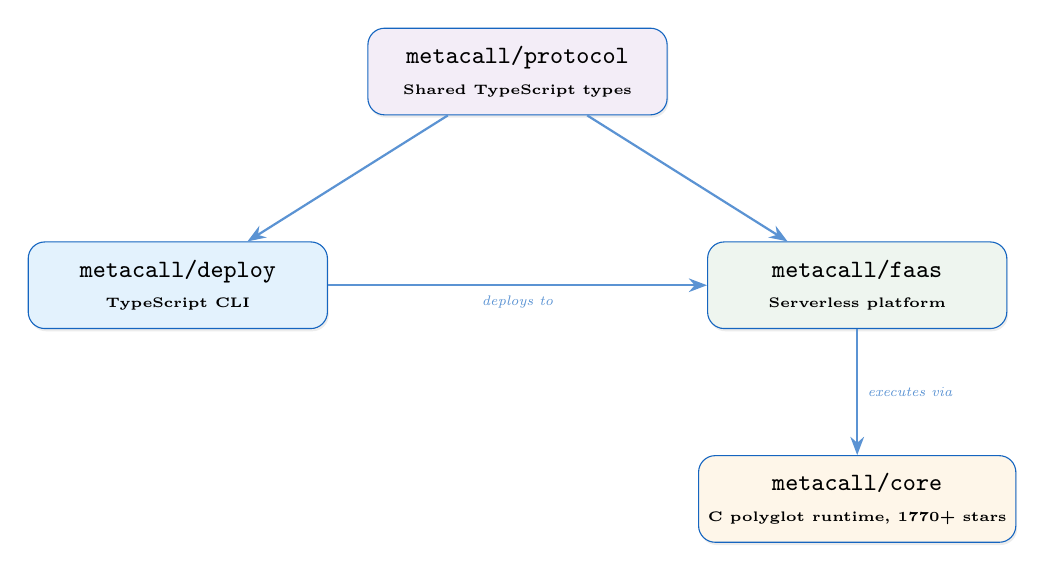
\begin{tikzpicture}[
  node distance=1.5cm and 1.8cm,
  pkg/.style={rectangle, draw=mcblue, fill=white,
              rounded corners=6pt,
              minimum width=3.8cm, minimum height=1.1cm,
              align=center, font=\small\bfseries,
              drop shadow={shadow xshift=0.5pt,
                           shadow yshift=-1pt, fill=gray!30}},
  arr/.style={-Stealth, thick, color=mcblue!70}
]
  \node[pkg, fill=mcpurple!8] (proto)
    {\texttt{metacall/protocol}\\
     {\tiny Shared TypeScript types}};
  \node[pkg, fill=mclight,
    below left=1.6cm and 0.5cm of proto] (deploy)
    {\texttt{metacall/deploy}\\
     {\tiny TypeScript CLI}};
  \node[pkg, fill=mcgreen!8,
    below right=1.6cm and 0.5cm of proto] (faas)
    {\texttt{metacall/faas}\\
     {\tiny Serverless platform}};
  \node[pkg, fill=mcgold!10, below=1.6cm of faas] (core)
    {\texttt{metacall/core}\\
     {\tiny C polyglot runtime, 1770+ stars}};

  \draw[arr] (proto) -- (deploy);
  \draw[arr] (proto) -- (faas);
  \draw[arr] (deploy) --
    node[below, font=\tiny\itshape, sloped]{deploys to} (faas);
  \draw[arr] (faas) --
    node[right, font=\tiny\itshape]{executes via} (core);
\end{tikzpicture}
\caption{MetaCall ecosystem: protocol, deploy, faas, and core}
\end{figure}

\subsection{What Is MCP?}

The Model Context Protocol is an open standard created by Anthropic that
lets AI assistants interact with external tools through a standardized
interface. Think of it as a USB port for AI tools. An MCP server exposes
three primitives:

\begin{itemize}[leftmargin=1.5em, itemsep=2pt]
  \item \textbf{Tools} are actions the AI can invoke
        (``deploy this function'')
  \item \textbf{Resources} are data the AI can read
        (deployment metadata)
  \item \textbf{Prompts} are reusable templates
        for common workflows
\end{itemize}

\subsection{Why This Combination Matters}

MetaCall's FaaS is powerful, but right now it requires CLI commands or
direct HTTP calls. MCP bridges that gap: developers interact with
polyglot serverless functions through natural language in any AI tool.
The time from idea to deployed function drops from minutes to seconds.

This is exactly what the GSoC project description asks for:
\emph{``Implement a minimal project that can be used for Claude or
similar LLMs from Visual Studio Code or Antigravity that allows to
deploy functions, list the existing ones, or run them locally in
multiple languages.''}

\subsection{FaaS API Endpoints}

\begin{table}[H]
\centering
\rowcolors{2}{mcgray}{white}
\begin{tabularx}{\textwidth}{>{\ttfamily\small}l >{\ttfamily\small}l X}
  \toprule
  \rowcolor{mcblue!15}
  \textbf{Method} & \textbf{Endpoint} & \textbf{Purpose} \\
  \midrule
  GET  & /api/readiness       & Health check \\
  GET  & /api/inspect         & List all deployments \\
  POST & /api/package/create  & Upload a zip package \\
  POST & /api/repository/add  & Clone a git repository \\
  POST & /api/deploy/create   & Create a deployment \\
  POST & /api/deploy/delete   & Delete a deployment \\
  POST & /api/deploy/logs     & Fetch deployment logs \\
  \bottomrule
\end{tabularx}
\caption{MetaCall FaaS API endpoints}
\end{table}

% ============================================================
%  5. PROJECT PROPOSAL
% ============================================================
\newpage
\section{Project Proposal}

\subsection{Problem Statement}

MetaCall's polyglot FaaS platform currently requires developers to use a
CLI or raw HTTP requests. In 2026, where AI coding assistants are
integral to every developer's workflow, there is no standard way to
interact with MetaCall through an AI interface. Project \#8 fixes this.

\subsection{Proposed Solution}

Build a production-grade MCP server in TypeScript that exposes MetaCall
Deploy and FaaS capabilities as MCP tools, resources, and prompts. This
enables any MCP-compatible AI assistant (Copilot, Claude, Antigravity)
to interact with MetaCall through natural language.

\subsection{Full Architecture}

\begin{figure}[H]
\centering
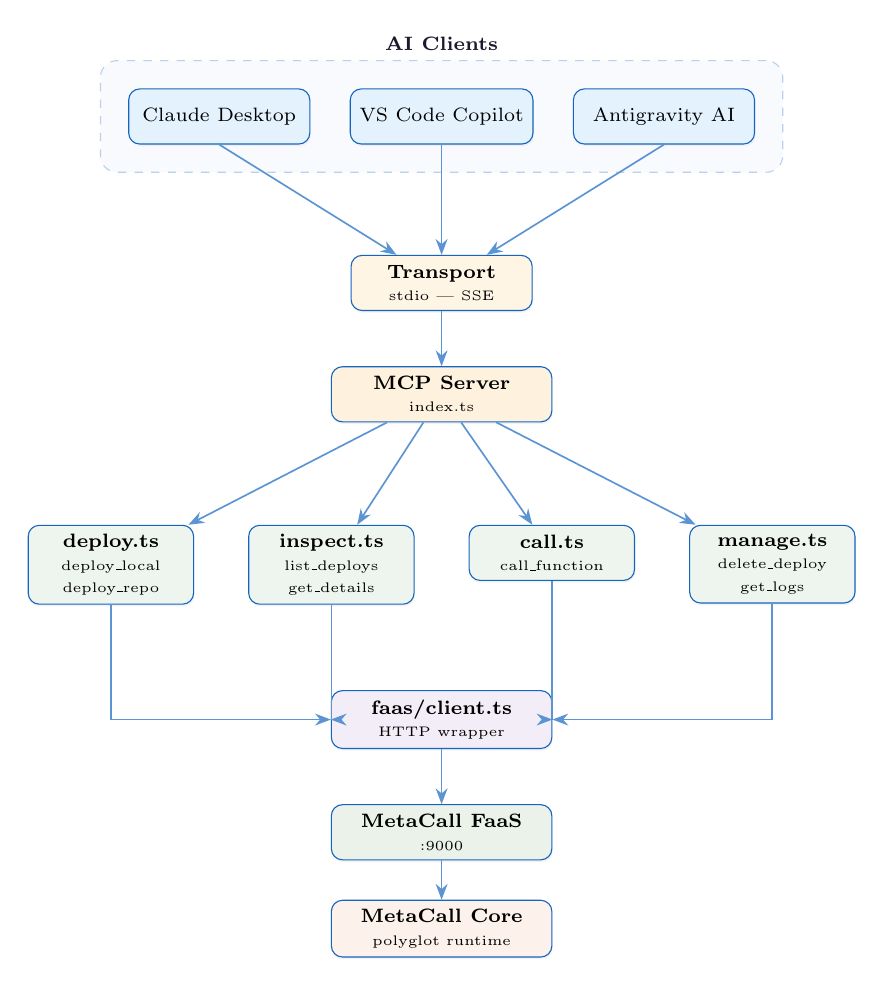
\begin{tikzpicture}[
  node distance=0.7cm and 0.5cm,
  layer/.style={rectangle, draw=mcblue!30, fill=mcblue!3,
                dashed, rounded corners=6pt, inner sep=10pt},
  box/.style={rectangle, draw=mcblue, fill=white,
              rounded corners=4pt,
              minimum width=2.3cm, minimum height=0.7cm,
              align=center, font=\scriptsize,
              drop shadow={shadow xshift=0.3pt,
                           shadow yshift=-0.8pt, fill=gray!20}},
  arr/.style={-Stealth, semithick, color=mcblue!70}
]
  \node[box, fill=mclight] (claude)   {Claude Desktop};
  \node[box, fill=mclight,
    right=0.5cm of claude]  (copilot)  {VS Code Copilot};
  \node[box, fill=mclight,
    right=0.5cm of copilot] (antigrav) {Antigravity AI};

  \begin{scope}[on background layer]
    \node[layer, fit=(claude)(copilot)(antigrav),
      label={[font=\scriptsize\bfseries\color{mcdark}]%
              above:AI Clients}] {};
  \end{scope}

  \node[box, fill=mcgold!12,
        below=1.4cm of copilot] (transport)
    {\textbf{Transport}\\{\tiny stdio | SSE}};

  \draw[arr] (claude.south)   -- (transport);
  \draw[arr] (copilot.south)  -- (transport);
  \draw[arr] (antigrav.south) -- (transport);

  \node[box, fill=mcgold!15, minimum width=2.8cm,
        below=0.7cm of transport] (server)
    {\textbf{MCP Server}\\{\tiny index.ts}};
  \draw[arr] (transport) -- (server);

  \node[box, fill=mcgreen!8, minimum width=2.1cm,
        below=1.3cm of server, xshift=-4.2cm] (t1)
    {\textbf{deploy.ts}\\{\tiny deploy\_local}\\
     {\tiny deploy\_repo}};
  \node[box, fill=mcgreen!8, minimum width=2.1cm,
        below=1.3cm of server, xshift=-1.4cm] (t2)
    {\textbf{inspect.ts}\\{\tiny list\_deploys}\\
     {\tiny get\_details}};
  \node[box, fill=mcgreen!8, minimum width=2.1cm,
        below=1.3cm of server, xshift=1.4cm] (t3)
    {\textbf{call.ts}\\{\tiny call\_function}};
  \node[box, fill=mcgreen!8, minimum width=2.1cm,
        below=1.3cm of server, xshift=4.2cm] (t4)
    {\textbf{manage.ts}\\{\tiny delete\_deploy}\\
     {\tiny get\_logs}};

  \draw[arr] (server) -- (t1);
  \draw[arr] (server) -- (t2);
  \draw[arr] (server) -- (t3);
  \draw[arr] (server) -- (t4);

  \node[box, fill=mcpurple!8, minimum width=2.8cm,
        below=3.4cm of server] (client)
    {\textbf{faas/client.ts}\\{\tiny HTTP wrapper}};

  \draw[arr] (t1.south) |- (client);
  \draw[arr] (t2.south) |- (client);
  \draw[arr] (t3.south) |- (client);
  \draw[arr] (t4.south) |- (client);

  \node[box, fill=mcgreen!10, minimum width=2.8cm,
        below=0.7cm of client] (faas)
    {\textbf{MetaCall FaaS}\\{\tiny :9000}};
  \node[box, fill=mcorange!8, minimum width=2.8cm,
        below=0.5cm of faas] (core)
    {\textbf{MetaCall Core}\\{\tiny polyglot runtime}};

  \draw[arr] (client) -- (faas);
  \draw[arr] (faas)   -- (core);
\end{tikzpicture}
\caption{Full production architecture of the MCP server}
\end{figure}

\newpage
\subsection{Repository Structure}

\begin{lstlisting}[language={}, numbers=none, frame=none,
  backgroundcolor=\color{mcgray},
  basicstyle=\ttfamily\small,
  caption={Proposed final project structure}]
metacall-mcp/
  src/
    index.ts            # MCP server entry point
    tools/
      deploy.ts         # deploy_local, deploy_repository
      inspect.ts        # list_deployments, get_details
      call.ts           # call_function
      manage.ts         # delete_deployment, get_logs, env
    transport/
      stdio.ts          # VS Code, Claude Desktop
      sse.ts            # Antigravity, web-based tools
    faas/
      client.ts         # HTTP client for all FaaS APIs
      types.ts          # Types (uses metacall/protocol)
    resources/
      deployments.ts    # MCP Resources: deployment data
    prompts/
      templates.ts      # MCP Prompt templates
  tests/integration/
    deploy.test.ts      # Jest tests for deploy tools
    inspect.test.ts     # Jest tests for inspect tools
    call.test.ts        # Jest tests for call tools
  docs/
    README.md           # Setup, configuration, usage
    INTEGRATION.md      # AI client integration guide
  package.json
  tsconfig.json
\end{lstlisting}

\subsection{MCP Tools: Complete Specification}

\begin{table}[H]
\centering
\rowcolors{2}{mcgray}{white}
\begin{tabularx}{\textwidth}{>{\ttfamily\bfseries\footnotesize}p{3.4cm} X c}
  \toprule
  \rowcolor{mcblue!15}
  \textbf{Tool} & \textbf{Description} & \textbf{Phase} \\
  \midrule
  list\_deployments &
    List all deployments with status, version, prefix & 1 \\
  deploy\_local &
    Deploy from a local directory path & 1 \\
  call\_function &
    Call any deployed function with arguments & 1 \\
  deploy\_repository &
    Deploy from a GitHub repository URL & 2 \\
  get\_function\_details &
    Get function signature, parameters, types & 2 \\
  delete\_deployment &
    Delete a deployment by name & 2 \\
  get\_logs &
    Fetch logs for a specific deployment & 2 \\
  set\_env\_vars &
    Set environment variables for a deployment & 3 \\
  \bottomrule
\end{tabularx}
\caption{All MCP tools across implementation phases}
\end{table}

\subsection{Key Implementation Details}

\subsubsection{Dual Transport Support}

\begin{figure}[H]
\centering
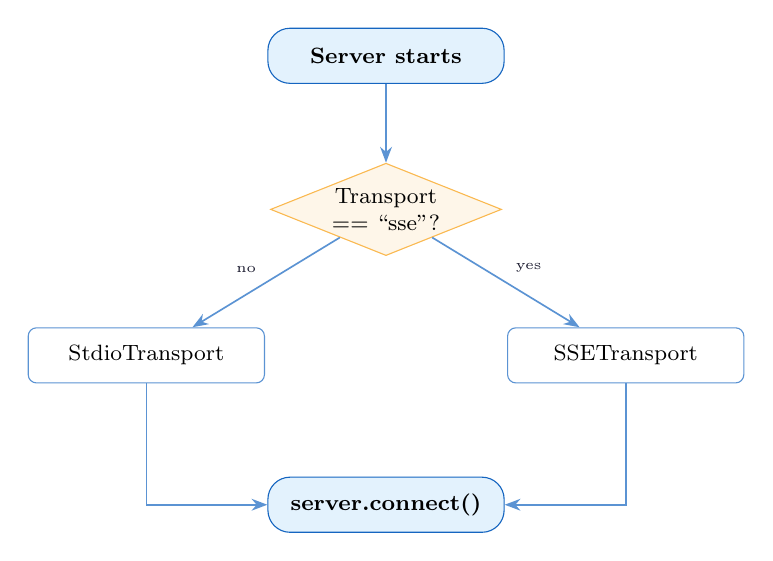
\begin{tikzpicture}[
  node distance=0.9cm,
  startstop/.style={rectangle, rounded corners=8pt,
    draw=mcblue, fill=mclight,
    minimum width=3cm, minimum height=0.7cm,
    align=center, font=\footnotesize\bfseries},
  process/.style={rectangle, rounded corners=3pt,
    draw=mcblue!70, fill=white,
    minimum width=3cm, minimum height=0.7cm,
    align=center, font=\footnotesize},
  decision/.style={diamond, draw=mcgold!80, fill=mcgold!10,
    minimum width=1.4cm, minimum height=0.7cm,
    align=center, font=\footnotesize,
    inner sep=1pt, aspect=2.5},
  arr/.style={-Stealth, semithick, color=mcblue!70},
  lbl/.style={font=\tiny, text=mcdark}
]
  \node[startstop] (start) {Server starts};
  \node[decision, below=1cm of start] (check)
    {Transport\\== ``sse''?};
  \node[process, below left=1.2cm and 0.8cm of check] (stdio)
    {StdioTransport};
  \node[process, below right=1.2cm and 0.8cm of check] (sse)
    {SSETransport};
  \node[startstop, below=2.8cm of check] (connect)
    {server.connect()};

  \draw[arr] (start) -- (check);
  \draw[arr] (check) -- node[lbl, above left]{no} (stdio);
  \draw[arr] (check) -- node[lbl, above right]{yes} (sse);
  \draw[arr] (stdio) |- (connect);
  \draw[arr] (sse)   |- (connect);
\end{tikzpicture}
\caption{Flowchart: Transport selection logic}
\end{figure}

\begin{lstlisting}[caption={Transport selection in index.ts},
  style=tsStyle]
import { StdioServerTransport }
  from '@modelcontextprotocol/sdk/server/stdio.js';
import { SSEServerTransport }
  from '@modelcontextprotocol/sdk/server/sse.js';

const transport =
  process.env.MCP_TRANSPORT === 'sse'
    ? new SSEServerTransport('/sse', response)
    : new StdioServerTransport();

await server.connect(transport);
\end{lstlisting}

\subsubsection{Repository Deployment Tool}

\begin{figure}[H]
\centering
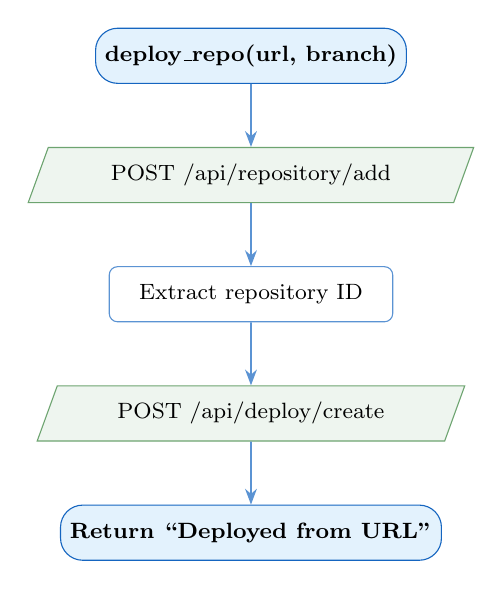
\begin{tikzpicture}[
  node distance=0.8cm,
  startstop/.style={rectangle, rounded corners=8pt,
    draw=mcblue, fill=mclight,
    minimum width=3.6cm, minimum height=0.7cm,
    align=center, font=\footnotesize\bfseries},
  io/.style={trapezium, trapezium left angle=70,
    trapezium right angle=110,
    draw=mcgreen!70, fill=mcgreen!8,
    minimum width=3cm, minimum height=0.7cm,
    align=center, font=\footnotesize},
  process/.style={rectangle, rounded corners=3pt,
    draw=mcblue!70, fill=white,
    minimum width=3.6cm, minimum height=0.7cm,
    align=center, font=\footnotesize},
  arr/.style={-Stealth, semithick, color=mcblue!70}
]
  \node[startstop] (start) {deploy\_repo(url, branch)};
  \node[io, below=of start] (add) {POST /api/repository/add};
  \node[process, below=of add] (getid) {Extract repository ID};
  \node[io, below=of getid] (deploy) {POST /api/deploy/create};
  \node[startstop, below=of deploy] (done)
    {Return ``Deployed from URL''};

  \draw[arr] (start) -- (add);
  \draw[arr] (add)   -- (getid);
  \draw[arr] (getid) -- (deploy);
  \draw[arr] (deploy) -- (done);
\end{tikzpicture}
\caption{Flowchart: deploy\_repository workflow}
\end{figure}

\begin{lstlisting}[caption={deploy\_repository tool}, style=tsStyle]
server.tool('deploy_repository', {
  repoUrl: z.string()
    .describe('GitHub repository URL'),
  branch:  z.string().default('main'),
  plan:    z.string().default('Essential')
}, async ({ repoUrl, branch, plan }) => {
  const { id } = await faas.post(
    '/api/repository/add',
    { url: repoUrl, branch }
  );
  const result = await faas.post(
    '/api/deploy/create',
    { id, resourceType: 'repository', plan }
  );
  return {
    content: [{
      type: 'text',
      text: `Deployed from ${repoUrl}`
    }]
  };
});
\end{lstlisting}

\subsubsection{MCP Resources}

\begin{lstlisting}[caption={Deployment resource registration},
  style=tsStyle]
server.resource(
  'deployments',
  'metacall://deployments',
  async (uri) => {
    const data = await faas.get('/api/inspect');
    return {
      contents: [{
        uri: uri.href,
        mimeType: 'application/json',
        text: JSON.stringify(data, null, 2)
      }]
    };
  }
);
\end{lstlisting}

\subsubsection{End-to-End Request Flow}

\begin{figure}[H]
\centering
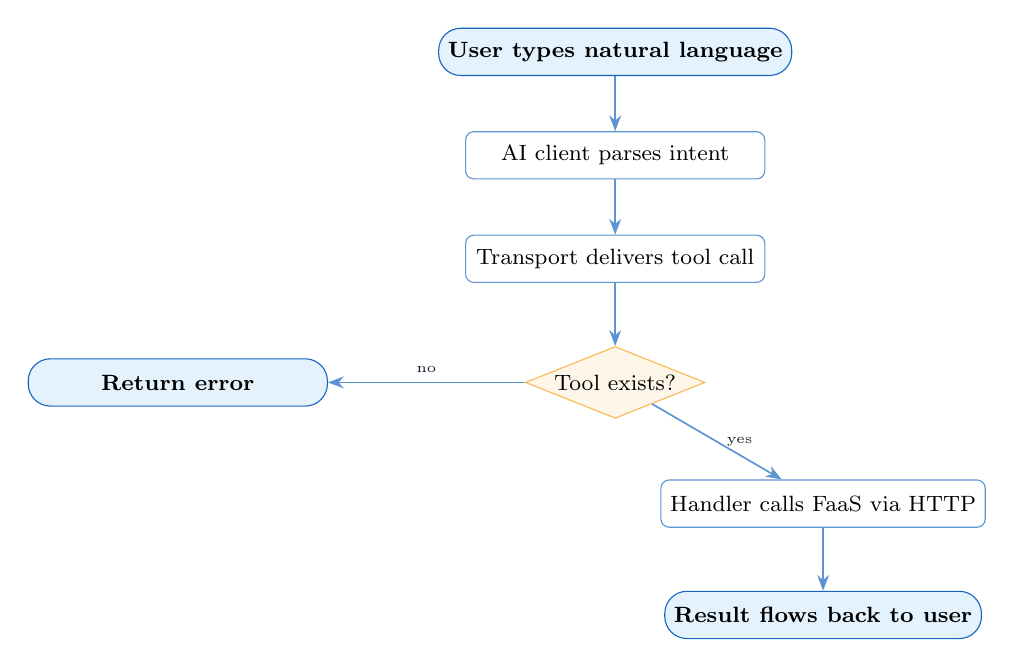
\begin{tikzpicture}[
  node distance=0.7cm,
  startstop/.style={rectangle, rounded corners=8pt,
    draw=mcblue, fill=mclight,
    minimum width=3.8cm, minimum height=0.6cm,
    align=center, font=\footnotesize\bfseries},
  process/.style={rectangle, rounded corners=3pt,
    draw=mcblue!70, fill=white,
    minimum width=3.8cm, minimum height=0.6cm,
    align=center, font=\footnotesize},
  decision/.style={diamond, draw=mcgold!80, fill=mcgold!10,
    minimum width=1.4cm, minimum height=0.6cm,
    align=center, font=\footnotesize,
    inner sep=1pt, aspect=2.5},
  arr/.style={-Stealth, semithick, color=mcblue!70},
  lbl/.style={font=\tiny, text=mcdark}
]
  \node[startstop] (start) {User types natural language};
  \node[process, below=of start] (parse) {AI client parses intent};
  \node[process, below=of parse] (route)
    {Transport delivers tool call};
  \node[decision, below=0.8cm of route] (check) {Tool exists?};
  \node[process, below right=1cm and 0cm of check] (exec)
    {Handler calls FaaS via HTTP};
  \node[startstop, below=0.8cm of exec] (result)
    {Result flows back to user};
  \node[startstop, left=2.5cm of check] (err) {Return error};

  \draw[arr] (start)  -- (parse);
  \draw[arr] (parse)  -- (route);
  \draw[arr] (route)  -- (check);
  \draw[arr] (check)  -- node[lbl, right]{yes} (exec);
  \draw[arr] (check)  -- node[lbl, above]{no} (err);
  \draw[arr] (exec)   -- (result);
\end{tikzpicture}
\caption{Flowchart: End-to-end MCP request lifecycle}
\end{figure}

\newpage
\section{Detailed Timeline (175 Hours)}

\begin{table}[H]
\centering
\rowcolors{2}{mcgray}{white}
\begin{tabularx}{\textwidth}{>{\bfseries\small}p{1.6cm} >{\small}p{2.2cm} X >{\small}r}
  \toprule
  \rowcolor{mcblue!15}
  \textbf{Phase} & \textbf{Dates} & \textbf{Deliverables} & \textbf{Hrs} \\
  \midrule
  Bonding & May 8--26 &
    Deep-dive into \texttt{metacall/protocol} types.
    Align architecture with mentors. Set up CI/CD.
    Write design doc. & 20 \\
  \midrule
  Phase 1 & May 27 -- Jun 16 &
    Core server scaffold.
    \texttt{list\_deployments}, \texttt{deploy\_local},
    \texttt{call\_function}. stdio transport.
    Basic README. Unit tests. & 45 \\
  \midrule
  Phase 2 & Jun 17 -- Jul 14 &
    \texttt{deploy\_repository},
    \texttt{get\_function\_details},
    \texttt{delete\_deployment}, \texttt{get\_logs}.
    MCP Resources. SSE transport.
    Claude Desktop integration. & 50 \\
  \midrule
  Midterm & Jul 14 &
    Phase 1 and 2 working, tested, documented. & -- \\
  \midrule
  Phase 3 & Jul 15 -- Aug 4 &
    Env variable support. MCP Prompt templates.
    Antigravity integration. npm publish setup.
    Integration tests with Jest. & 40 \\
  \midrule
  Phase 4 & Aug 5--25 &
    Full docs (README, INTEGRATION guide).
    Official MetaCall docs integration.
    Demo video. Final PR review. & 20 \\
  \midrule
  \rowcolor{mcblue!8}
  \textbf{Total} & & & \textbf{175} \\
  \bottomrule
\end{tabularx}
\caption{GSoC 2026 project timeline}
\end{table}

\textbf{Weekly rhythm:} I plan to commit 25 to 30 hours per week. I will
post weekly progress updates publicly, as agreed with MetaCall's
mentorship process. No planned vacations during the program.

\begin{figure}[H]
\centering
\includegraphics[width=\textwidth, keepaspectratio]{image.png}
\caption{Project timeline snapshot}
\label{fig:timeline-snapshot}
\end{figure}

% Force next major section to a brand new page
\clearpage

% ============================================================
%  7. BENEFITS
% ============================================================


% Section 7 starts from a brand-new page 
\clearpage
\section{Benefits to the Community}

\subsection{For MetaCall}

\begin{itemize}[leftmargin=1.5em, itemsep=3pt]
  \item Makes MetaCall \textbf{AI-native}: the first polyglot FaaS
        with full MCP support.
  \item Lowers the barrier to entry. Developers deploy polyglot
        functions without learning the CLI or API docs.
  \item Positions MetaCall as a leader at the intersection of AI
        tooling and polyglot computing.
  \item Directly fulfills every stated outcome of Project \#8.
\end{itemize}

\subsection{For the Open Source Community}

\begin{itemize}[leftmargin=1.5em, itemsep=3pt]
  \item Published as an \textbf{npm package} for immediate use.
  \item Reference implementation of an MCP server wrapping a cloud
        API, useful for anyone learning MCP.
  \item Integrates with Antigravity, extending reach beyond VS Code.
\end{itemize}

\subsection{For Developers}

A developer will be able to type:
\emph{``Deploy my Python flask app from github.com/me/myapp and call
the predict function with input 42''}
and have it work. No CLI. No API docs. Just natural language.


% ============================================================
%  8. RELATED WORK
% ============================================================
\section{Related Work and Differentiation}

\begin{table}[H]
\centering
\rowcolors{2}{mcgray}{white}
\begin{tabularx}{\textwidth}{l X X}
  \toprule
  \rowcolor{mcblue!15}
  \textbf{Project} & \textbf{What it does} &
  \textbf{How mine differs} \\
  \midrule
  AWS Lambda MCP & MCP for AWS Lambda &
    Not polyglot, not open source \\
  Vercel AI SDK & AI tools for Vercel &
    No polyglot runtime support \\
  My PoC & Working MCP for MetaCall &
    Only stdio, 3 tools, no tests \\
  \textbf{This project} & \textbf{Full MCP server} &
    \textbf{8 tools, both transports, tested, docs, npm-published} \\
  \bottomrule
\end{tabularx}
\caption{Comparison with existing work}
\end{table}

% ============================================================
%  9. WHY ME
% ============================================================
\newpage
\section{Why I Am the Right Person for This}

\begin{highlightbox}
Most applicants write proposals. I wrote \textbf{code first}.
\end{highlightbox}

\begin{enumerate}[leftmargin=1.5em, itemsep=5pt]
  \item \textbf{Working proof-of-concept already built.}
        I have a functioning MCP server that delivers the core
        expected outcome of Project \#8. Not theoretical.

  \item \textbf{Mentor validation.}
        viferga (MetaCall mentor) watched my demo and said
        ``awesome mate.'' Mostafa Wael Kamal (Project \#8
        mentor) has reviewed my work.

  \item \textbf{I know the codebase.}
        I read \texttt{metacall/deploy},
        \texttt{metacall/faas}, and
        \texttt{metacall/protocol}. I found two
        undocumented bugs. I submitted a PR following
        maintainer feedback.

  \item \textbf{Strong algorithmic foundation.}
        Ranked 3rd in DSA and 2nd in AI/ML in my college.
        Two years of competitive programming.

  \item \textbf{Proven hackathon winner.}
        1st Place at Build with Gemini $\times$ MLH
        international hackathon with MediMind.

  \item \textbf{Domain expertise.}
        AI/ML background (LLM integration, OpenAI API,
        multimodal systems) directly relevant to MCP.

  \item \textbf{Realistic proposal.}
        The 175-hour timeline is based on hours already
        logged building the PoC and exploring the codebase.

  \item \textbf{Community engagement.}
        Joined MetaCall Discord, shared work proactively,
        engaged with mentors technically.
\end{enumerate}

% ============================================================
%  10. AVAILABILITY
% ============================================================
\section{Availability and Commitments}

\begin{itemize}[leftmargin=1.5em, itemsep=3pt]
  \item \textbf{Hours per week:} 25--30 hours, meeting
        the 175-hour target comfortably
  \item \textbf{Timezone:} IST (UTC+5:30), overlap with
        European and Asian mentors
  \item \textbf{Academic conflicts:} Semester exams in
        early June; will notify mentors two weeks ahead
        and compensate hours in adjacent weeks
  \item \textbf{Communication:} Available daily on Discord;
        email response within 24 hours
  \item \textbf{Other commitments:} No other GSoC
        applications. This is my only, focused proposal
  \item \textbf{Internet:} Stable broadband, no disruptions
\end{itemize}

% ============================================================
%  11. AI USAGE
% ============================================================
\section{AI Usage Disclosure}

In accordance with MetaCall's
\href{https://github.com/metacall/gsoc-2026/blob/main/AI-USAGE-POLICY.md}%
{AI Usage Policy}:

\begin{infobox}[AI Usage Disclosure]
AI tools (GitHub Copilot in agent mode) were used as writing and
structuring assistants during drafting of this proposal. All technical
descriptions, code snippets, architectural decisions, and contributions
described here reflect my own work, understanding, and implementations.
AI was not used to generate any code submitted to MetaCall repositories.
Every line of code in the PoC and PR \#200 was written, understood, and
tested by me personally.
\end{infobox}

% ============================================================
%  12. CONCLUSION
% ============================================================
\section{Conclusion}

MetaCall is solving a genuinely hard problem: making polyglot computing
feel as natural as single-language development. MCP support takes this
one step further, making polyglot serverless computing as natural as
typing a sentence to your AI assistant.

I have not just read about this project. I have built it, tested it,
shipped a PR, found bugs, and earned the praise of the project's
founder. I am ready to take this from proof-of-concept to a
production-grade, documented, and officially integrated tool that
benefits the entire MetaCall community.

I look forward to working with the MetaCall team this summer.

\vspace{2em}
\noindent\textbf{Swastik Prakash}\\
\href{mailto:swastikprakashofficial@gmail.com}%
{swastikprakashofficial@gmail.com}\\
\href{https://github.com/Swastik-Prakash1}%
{github.com/Swastik-Prakash1}

\end{document}
